\chapter{Process}
\label{processSec}
This project is largest project the author has solely been responsible for however, this does not define the project as a large project. Given the time frame which the project has to be completed in the author to come to the conclusion that there is no single process model that would fully suitable. The lack of one specific process gives the author the temptation adopt no process at all however, the lack of any rational structure is inappropriate for this project.

Rather than using one single process the author feels that he can modify existing processes in order to create a process which captures the principles required to create a logical process for this project. Agile methodologies specifically eXtreme Programming (XP) principles are often used in small development teams. XP places heavy importance on quality and responding to customer demands through the use of multiple iterations and a simple design process. Some argue that small development teams are using XP as a scapegoat for not adhering to a specific process or methodology. XP is still very much focused around a development team and there is constant deliberation about the adaptation of XP for single developer projects\cite{XP:forone}. There are XP principles which are well suited to this style of project for example, there is less emphasis on a heavy on design allowing for a more flexible development process. This has been vital for this project in particular as the proposed design had to be significantly changed during development (see section \ref{DesignSec}). The author feels that in a solo project, the ability to be flexible and independent of any concrete design is key to a successful project. As the author has created a brief design specification individually without the help of a specialised team (see appendix B) there is the possibility that there are some key elements missing which may not be noticed until the implementation stage. Capitalising on XP's flexibility reduces the impact of the exclusion of key features during design as it enables the author to easily adapt to system changes. 

The process used is a hybrid process containing relevant ideologies from other software development processes. In conjunction with XP principles discussed above, the author has decided that there has to be some planned process involved in the projects development. The idea behind using a planned approach as the main underlying process is because the author feels that solo projects often lose track of project goals and the documentation of such goals will remove this complication. This planned process won’t be as strict as it would be if a planned approach was the sole process being used for this project, instead the design and requirements phase will be much shorter than usual and will only cover the main requirements and overall system interactions. 

\begin{figure}[H]
\centering
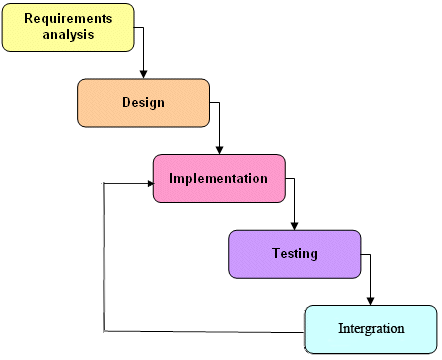
\includegraphics[scale=0.7]{Images/chapter3/waterfallmodel}
\caption[Waterfall Model Variant]{Variant of the Waterfall Model used in this project. Modified from source image \cite{waterfall:image}}
\label{fig:waterfall}
\end{figure}

Figure \ref{fig:waterfall} represents the variation of the waterfall model used for this project. The general waterfall structure has remained the same, the process starts off with a problem analysis stage which is reflected in appendix A and chapter \ref{chap:analysis}. The introduction of the XP principles puts less emphasis on the design stage. This is intended to remove the dependancy on any concrete design. The main adaptation comes from the approach to implementation and testing, the inclusion of XP principles enables the author to be more flexible during the implementation process. This hybrid process enables the author to focus on the implementation and testing of any changes rather than focusing on redesigning the system to accommodate such changes, this saved tremendous amounts of time during development. Each change is handled in small sections rather than implementing several changes at once. Each change will be broken down into logical sections which will go through the implementation and testing process. Design is not completely disregarded, the author still has the option to design any new changes should he feel the need to. This process continues until the requirements define in appendix A have been adhered to. This hybrid process is based on the work by Tom Blanchard \cite{tblanch:diss}, the process is very effective for use in solo projects.
